\documentclass{article}
\usepackage{graphicx} % Required for inserting images
\usepackage{amsmath}
\usepackage{amssymb}
\usepackage{indentfirst}
\usepackage{float}
\usepackage{caption}
\usepackage[a4paper, total={6in, 10in}]{geometry}

\title{Mathcamp 2026 Qualifying Quiz Problem 3 Solution}
\author{Applicant ID: 25107}
\date{}

\begin{document}
	
	\maketitle
	
	\section*{Part a)}
	Assign coordinates to each square so that the square in the $x$-th column from the left and $y-$th row from the bottom has coordinates $(x, y)$. This means the fire starts at $(1, 1)$. Now, let $S_d$ be the set of squares on fire on the $d$-th diagonal on day $d$, where the $d$-th diagonal consists of all squares $(x, y)$ such that $x + y - 1 = d$. On day $d$, the furthest the fire can spread is diagonal $d$, so if $|S_d| \geq 1$ for all $d$, then it must be that the fire keeps spreading.
\begin{figure}[h]
    \centering
    \vspace{-0.3cm}
    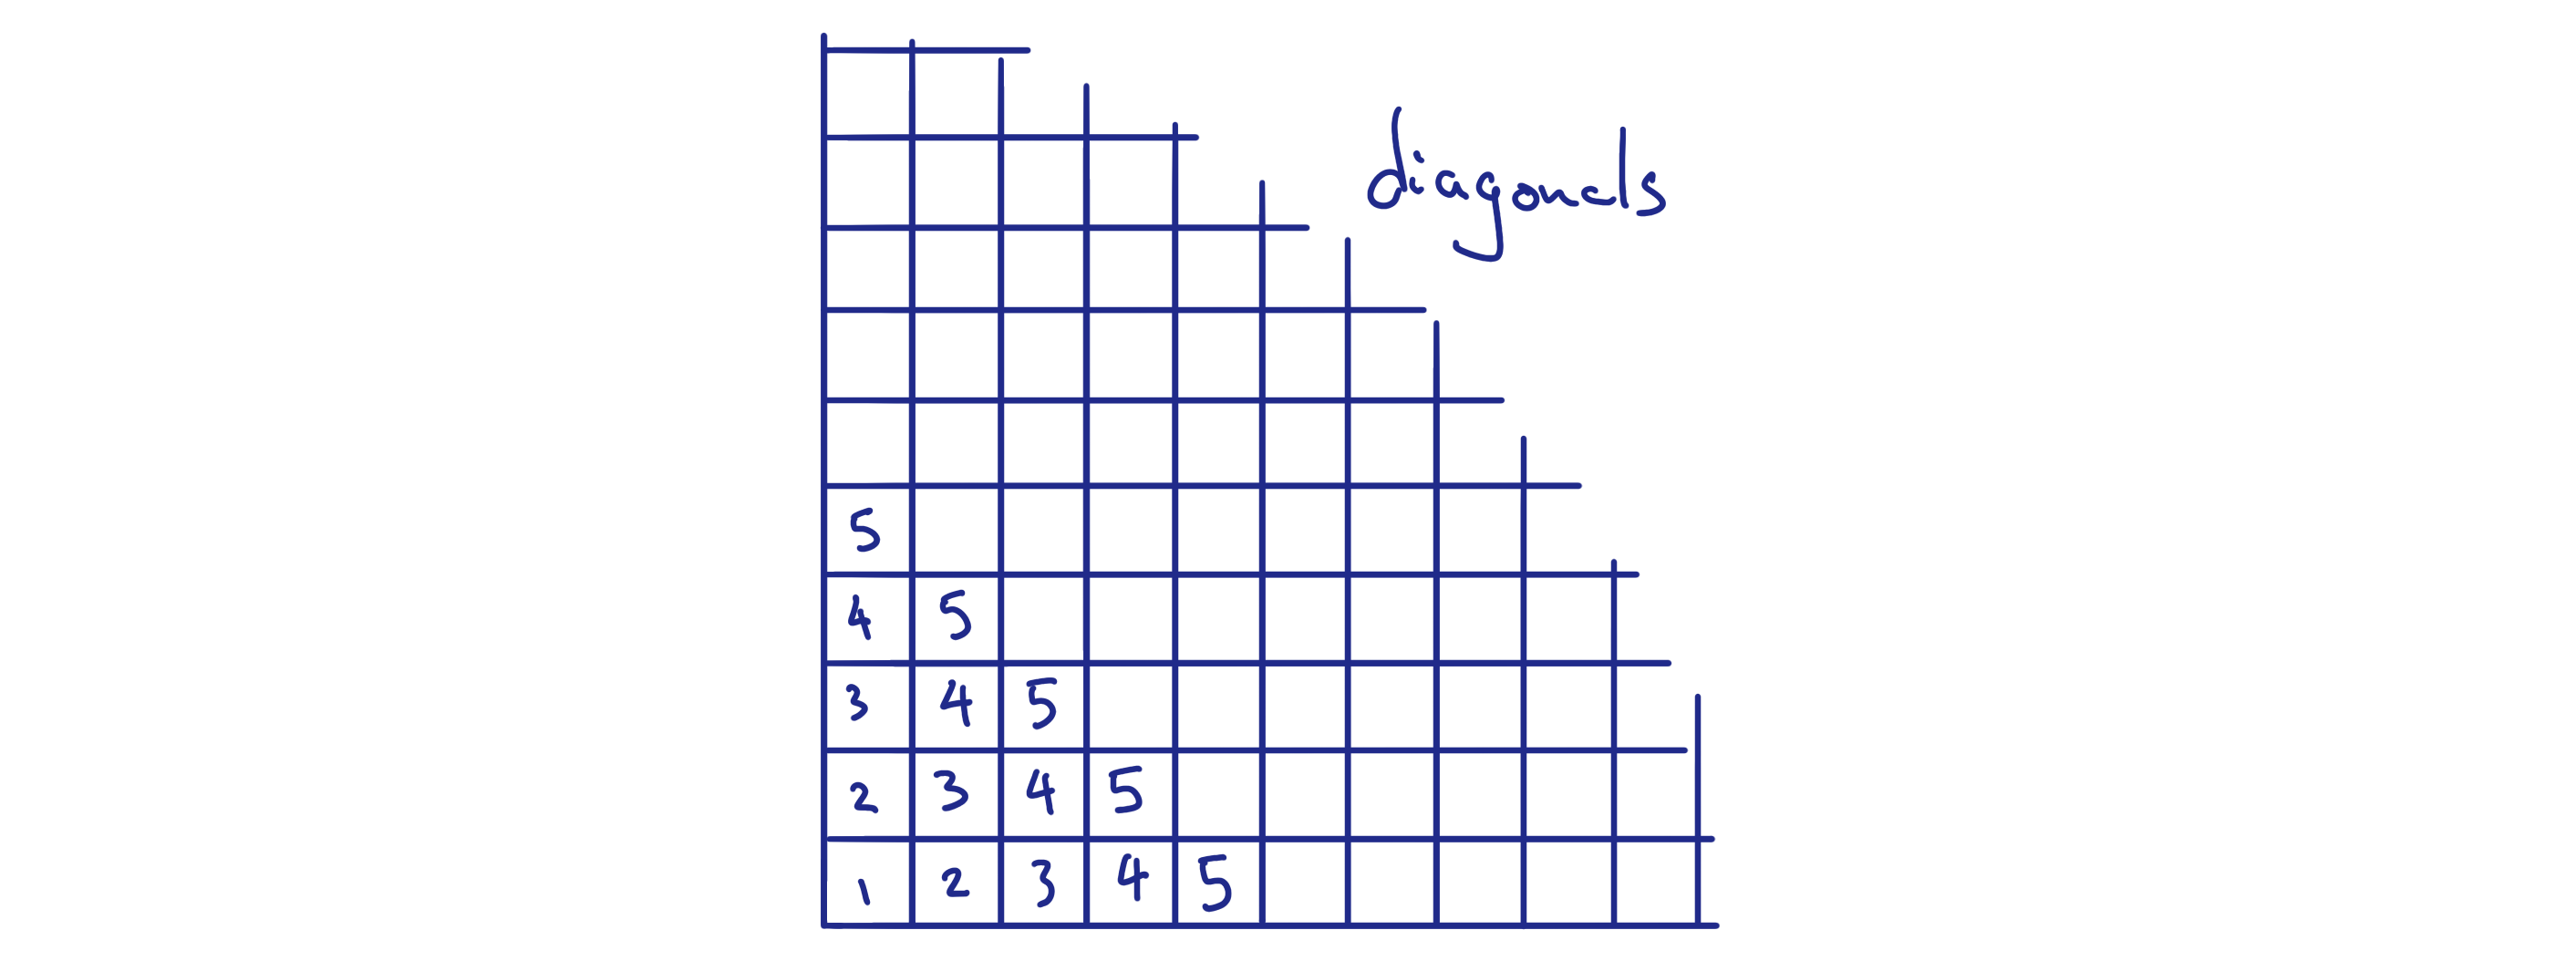
\includegraphics[width=14cm]{diagonals.png}
    \vspace{-0.3cm}
\end{figure}

	Consider now the situation where on day $d$, there are no protected squares on the $(d + 1)$-th diagonal. We first show that more than $|S_d|$ squares will catch fire on the $(d + 1)$-th diagonal. Consider the sets $$X = \{(x + 1, y)\mid (x, y) \in S_d\},\quad Y = \{(x, y + 1)\mid (x, y) \in S_d\},$$ which both contain $|S_d|$ squares. By considering some square in $S_d$ with the maximum $y$-coordinate, we see that $X$ and $Y$ are disjoint. As the number of squares that will catch fire on the $(d + 1)$-th diagonal is $|X\cup Y|$, the result follows.
\begin{figure}[h]
    \centering
    \vspace{-0.3cm}
    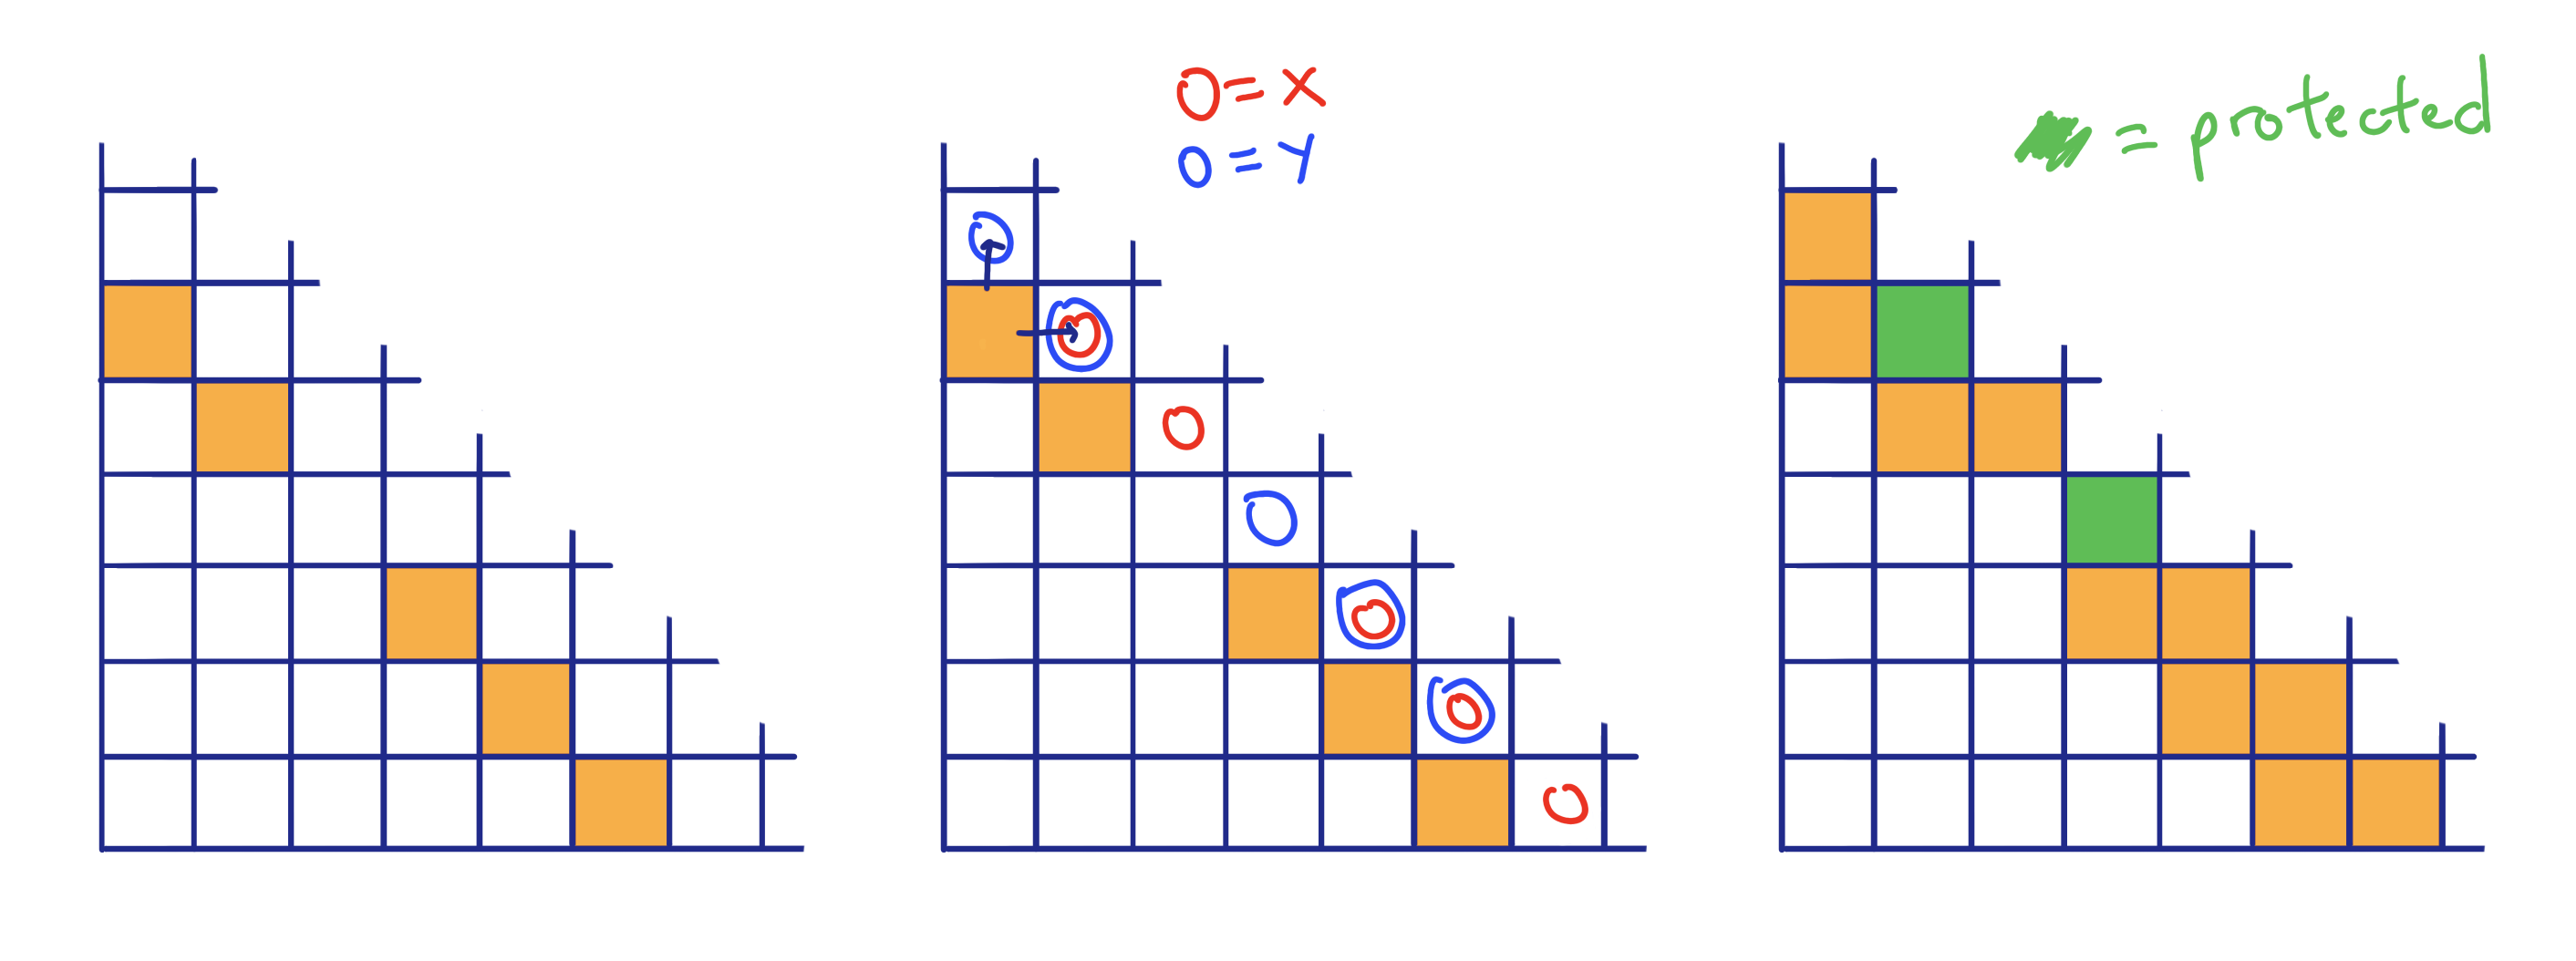
\includegraphics[width=14cm, trim = 0 0cm 0 0.5cm, clip]{expansion.png}
    \vspace{-0.3cm}
\end{figure}
    
	Now, let $P_d$ be the set of protected squares on the $d$-th diagonal on day $d$. We have that $$|S_{d + 1}| \geq |S_d| + 1 - |P_d|.$$ Therefore on day $D$,
	\begin{align*}
		|S_D| &\geq |S_{D - 1}| + 1 - |P_{D - 1}| \\
		&\geq |S_{D - 2}| + 1 - |P_{D - 2}| + 1 - |P_{D - 1}| \\
		&\vdots \\
		&\geq |S_0| + D - \sum_{i = 0}^{D - 1}|P_i| \geq 1 - D + D = 1.
	\end{align*}
	
	From this, we see that the fire never stops spreading.
	
	\section*{Part b)}
	Without loss of generality, let $n \leq m$. We claim that we must protect at least $n + 1$ squares on the first day, and proceed by induction on $n$. First, consider the base case where $n = 1$. From part a), we must protect more than one square on the first day to be able to cover all squares. However, protecting two squares on day one is sufficient, like so:
\begin{figure}[h]
    \centering
    \vspace{-0.3cm}
    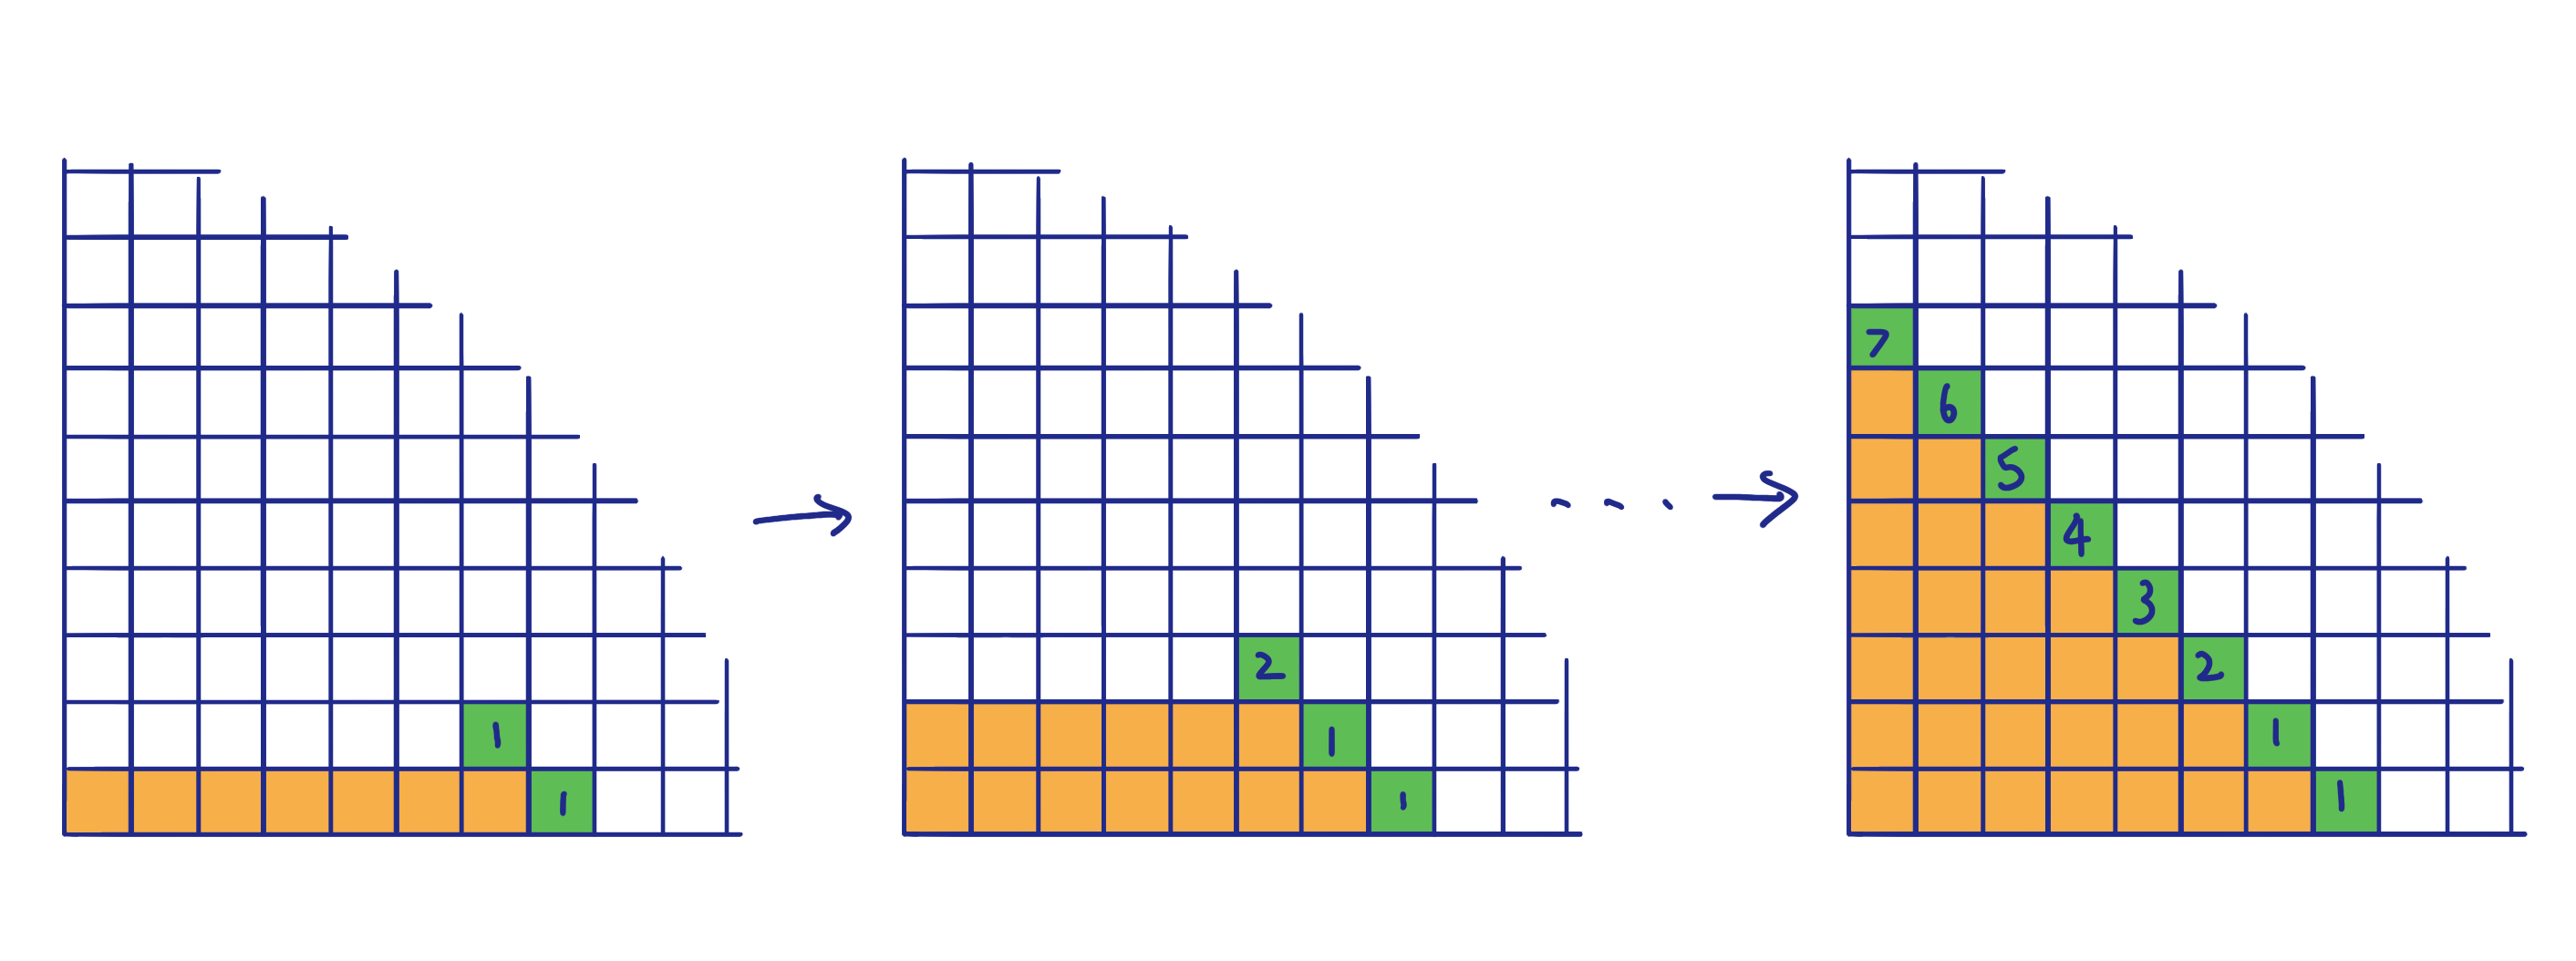
\includegraphics[width=15cm, trim = 0 1cm 0 1cm, clip]{linecase.png}
    \vspace{-0.3cm}
\end{figure}

	Now, assume that for $n < m$, we must protect at least $n + 1$ squares on the first day, and consider the situation starting with an $(n + 1)\times m$ grid on fire. To eventually stop the fire from spreading, we must contain both regions $A$ and $B$. By our inductive hypothesis, we must place $n + 1$ squares in region $A$. Suppose we contain the fire in region $A$ on day $D$. Then, we will have protected $n + D$ squares, so the greatest $x$-coordinate a protected square could have is $n + D$. However, as this requires only protecting squares in region $A$, on day $D + 1$, the fire in region $B$ will have spread to column $m + D > n + D$. This will create a `corner' as shown below, which is impossible to contain as shown in part a).
\begin{figure}[h]
    \centering
    \vspace{-0.3cm}
    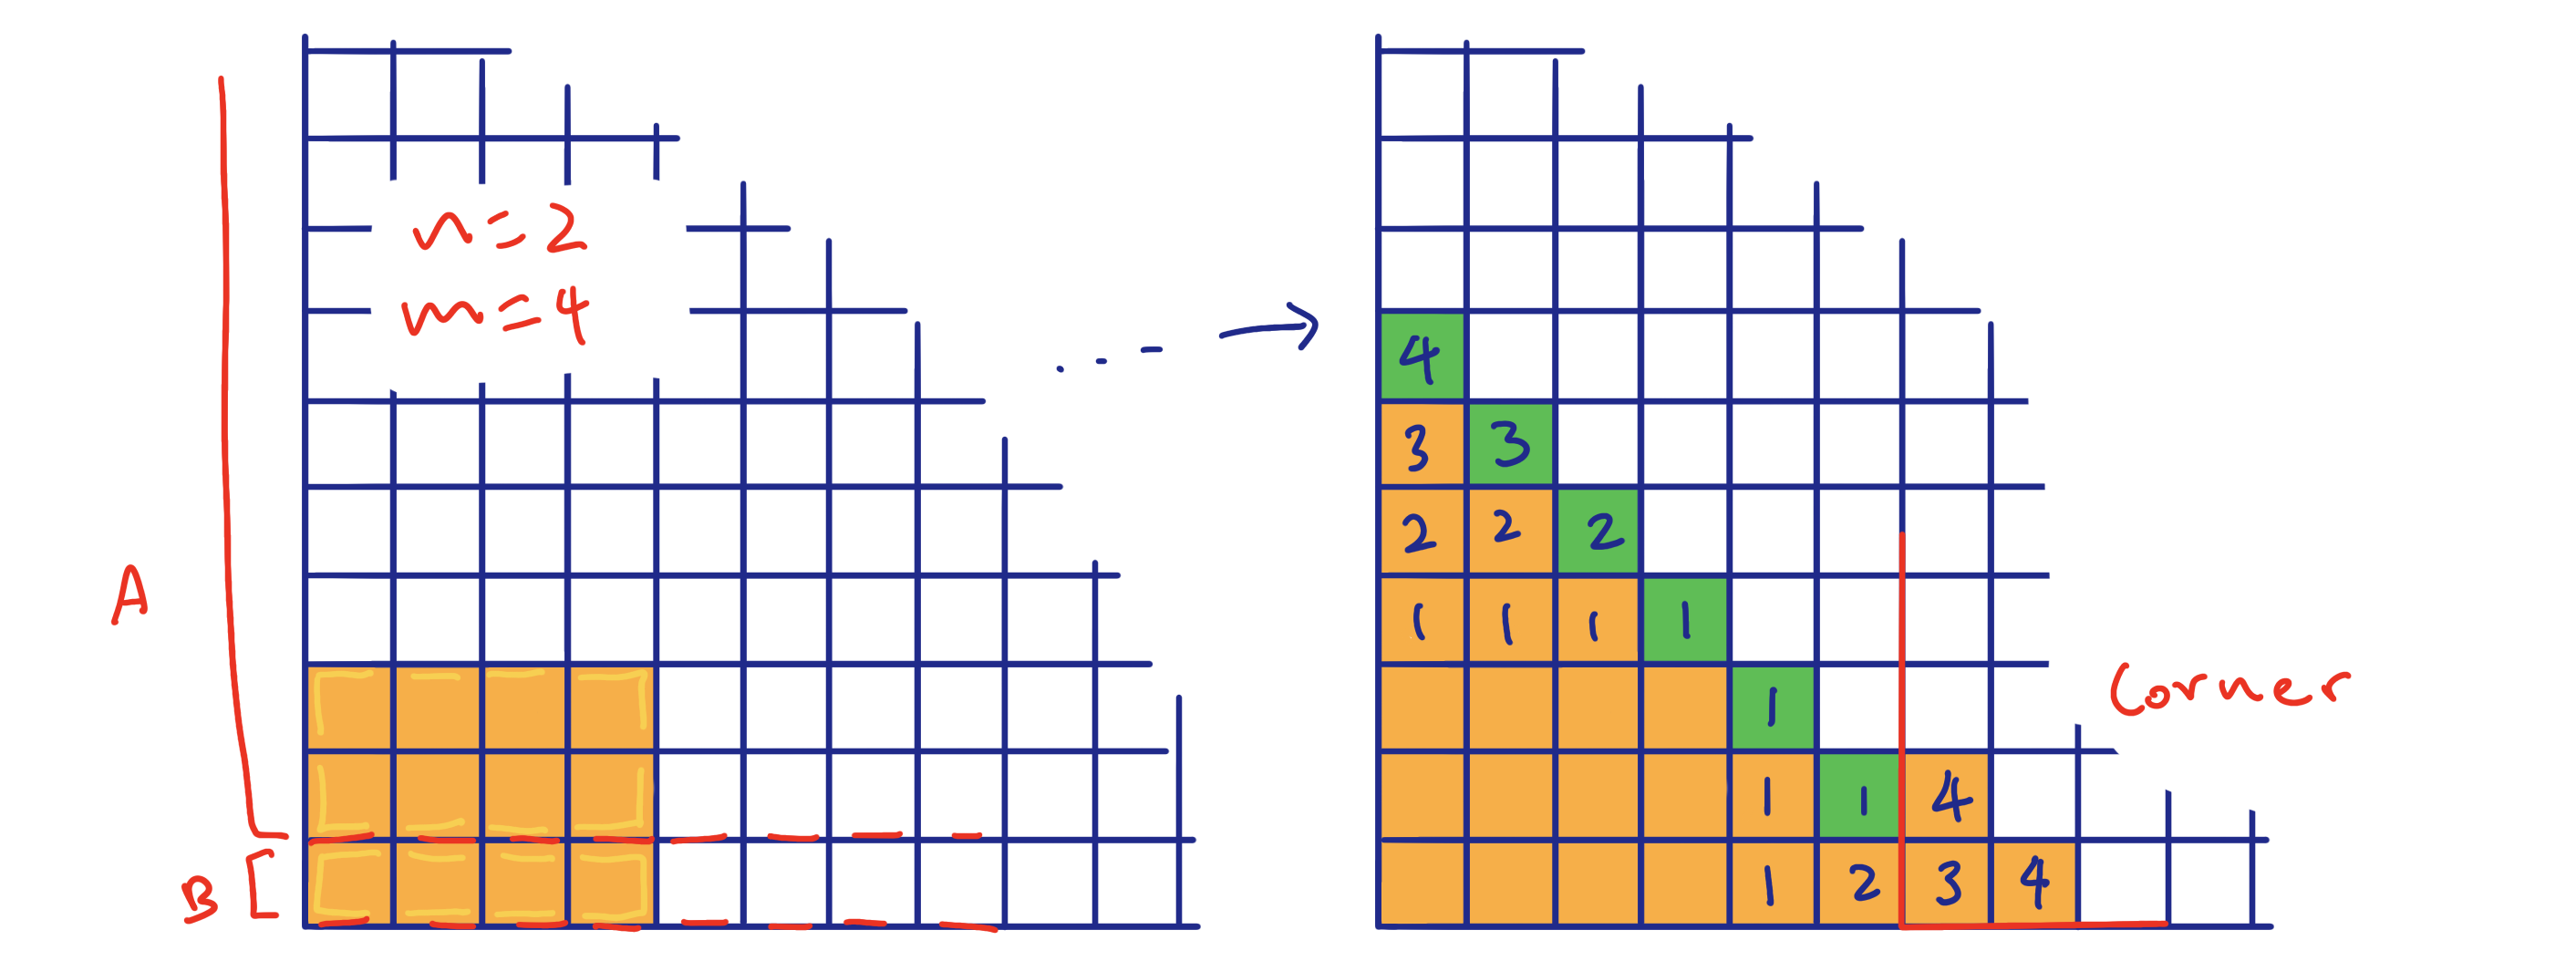
\includegraphics[width=14cm]{corner.png}
    \vspace{-0.3cm}
\end{figure}

	From this, we see that for an $(n + 1)\times m$ grid, protecting $n + 1$ squares on the first day is not enough. However, $n + 2$ squares is sufficient, like so:
\begin{figure}[H]
    \centering
    \vspace{-0.3cm}
    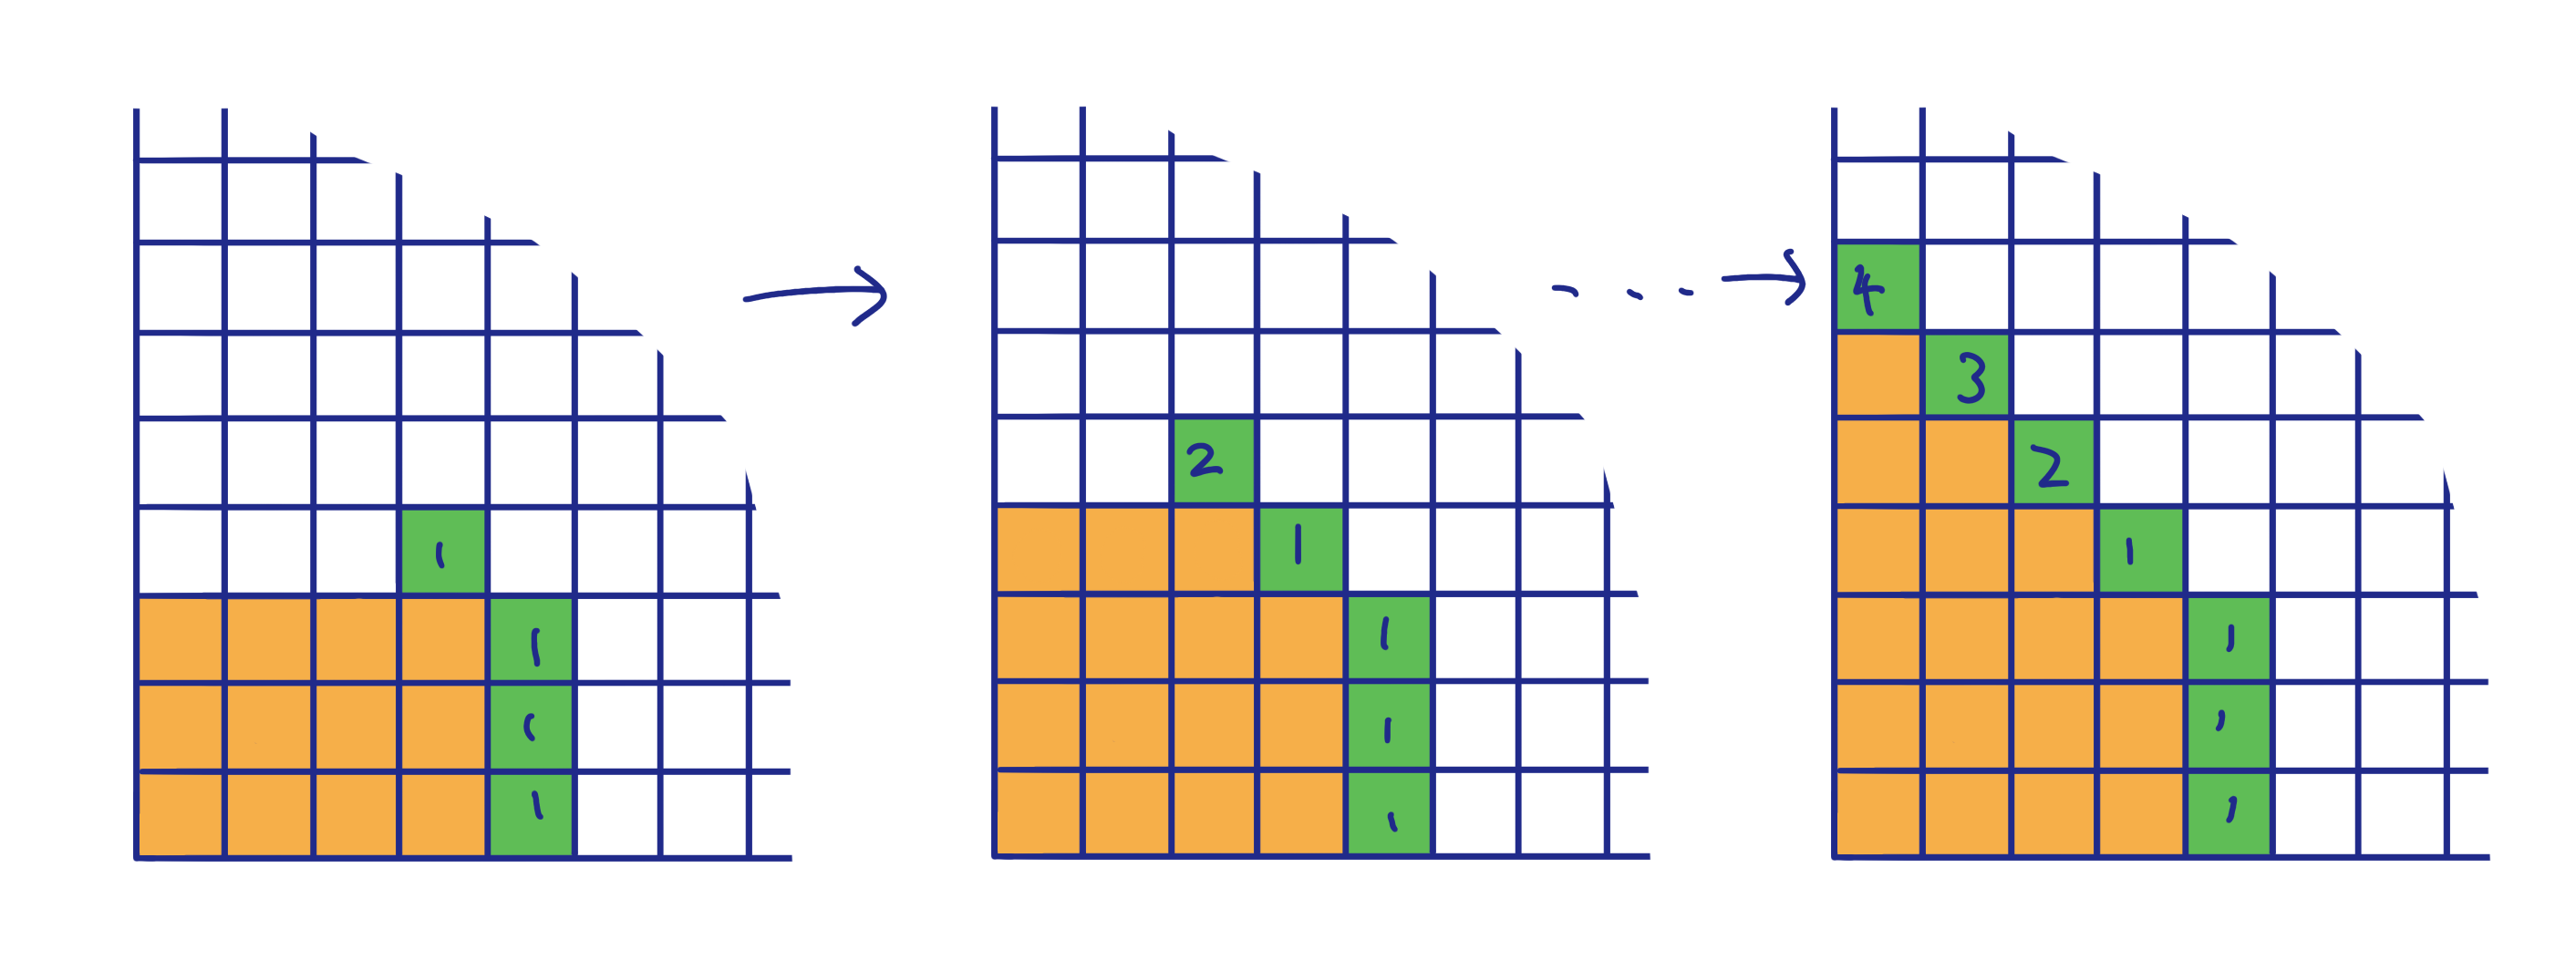
\includegraphics[width=15cm, trim = 0 1cm 0 1cm, clip]{solution.png}
    \vspace{-0.3cm}
\end{figure}
    
	Therefore, for an $n\times m$ grid, on the first day we must protect a minimum of $\min(n, m) + 1$ squares.
\end{document}